% That is the appendix. Just add stuff. that you do not want to include in the main report but still want to show. here.
% Name the label to for example "student03:appendix" if you are student 03 so that you can refer to your appendix in your ReportPart by using "\ref{student03:appendix}"
% No referencing in appendix implemented yet.

%%%%%%%%%%%%%%%%%%%%%  John Doe  %%%%%%%%%%%%%%%%%%%%%

\chapter{Appendix GPS measurements}
\label{studentxx:appendix}

\subsection*{Header of a position file}
% header position file 
\begin{verbatim}
 program   : RTKPOST ver.2.4.2
 inp file  : *.obs
 inp file  : lyrs07*0.18o
 inp file  : *.nav
 obs start : 2018/03/15 10:48:19.0 GPST (week1992 384499.0s)
 obs end   : 2018/03/15 11:19:49.0 GPST (week1992 386389.0s)
 pos mode  : static
 freqs     : L1+L2
 solution  : forward
 elev mask : 15.0 deg
 dynamics  : on
 tidecorr  : off
 ionos opt : iono-free
 tropo opt : saastamoinen
 ephemeris : broadcast
 navi sys  : gps glonass galileo qzss sbas
 amb res   : fix and hold
 amb glo   : on
 val thres : 3.0
 antenna1  :                       ( 0.0000  0.0000  0.0000)
 antenna2  :                       ( 0.0000  0.0000  0.0000)
 ref pos   : 78.228825638   15.397310064   495.6816
\end{verbatim}

\subsection*{Additional data}

% raw data from the measurements in the field
\begin{table}[h]
	\caption{Raw data collected in the field used for the stake correction.}
	\centering
	\begin{turn}{90}
		\scriptsize
		\begin{tabular}{lllllll}
\toprule
        Name &        Date & Antenna height [m] & Snow depth [m] & Inclination [deg] & Direction of Incl. [deg] & Distance Rover-Stake [m] \\
\midrule
    BL2-2016 &  15.03.2018 &               2.18 &            1.1 &                 3 &                      225 &                     0.18 \\
    BL2-2018 &  15.03.2018 &                0.6 &              0 &                 2 &                      270 &                        0 \\
    BL3-2016 &  15.03.2018 &                2.2 &           1.07 &                12 &                      270 &                      0.1 \\
    BL3-2018 &  15.03.2018 &                0.6 &              0 &                 0 &                        0 &                        0 \\
    BL4-2018 &  15.03.2018 &               0.92 &              0 &                 0 &                        0 &                        0 \\
  BL4-i-2016 &  15.03.2018 &               2.08 &           0.93 &                10 &                      270 &                     0.11 \\
 BL4-ii-2016 &  16.03.2018 &               1.25 &           1.25 &                10 &                      270 &                      0.2 \\
  BL5-i-2017 &  15.03.2018 &               1.32 &            1.1 &                 0 &                        0 &                        0 \\
 BL5-ii-2017 &    16.03.18 &               0.48 &            1.3 &                 0 &                        0 &                        0 \\
     T1-2018 &  13.03.2018 &               0.66 &              0 &                 0 &                        0 &                        0 \\
   T1-i-2017 &  11.03.2018 &                2.2 &            0.8 &                 9 &                      180 &                     0.15 \\
  T1-ii-2017 &  13.03.2018 &               2.15 &            0.8 &                10 &                      180 &                     0.17 \\
     T2-2016 &  15.03.2018 &               1.34 &           0.97 &                 0 &                        0 &                      0.1 \\
     T2-2018 &  13.03.2018 &               0.66 &              0 &                 5 &                      225 &                        0 \\
   T2-i-2017 &  11.03.2018 &               2.23 &              1 &                10 &                       90 &                      0.1 \\
  T2-ii-2017 &  13.03.2018 &                1.4 &              1 &                 5 &                      135 &                      0.1 \\
     T3-2017 &  11.03.2018 &               1.87 &           1.05 &                 0 &                        0 &                      0.1 \\
     T4-2016 &  11.03.2018 &               2.42 &            1.2 &                 5 &                        0 &                      0.1 \\
     T4-2018 &  13.03.2018 &               0.63 &              0 &                 0 &                        0 &                        0 \\
     T5-2016 &  11.03.2018 &               2.44 &           1.22 &                 8 &                        0 &                      0.1 \\
     T5-2018 &  15.03.2018 &               0.45 &              0 &                 0 &                        0 &                        0 \\
     T6-2016 &  11.03.2018 &                2.3 &           1.35 &                 4 &                      180 &                     0.15 \\
     T6-2018 &  15.03.2018 &               1.95 &            1.4 &                 0 &                        0 &                        0 \\
     T7-2015 &  13.03.2018 &               1.84 &            1.2 &                10 &                       45 &                      0.1 \\
     T7-2017 &  13.03.2018 &               0.98 &           1.21 &                 0 &                        0 &                        0 \\
     T8-2017 &  13.03.2018 &               2.09 &            0.7 &                 5 &                      180 &                      0.1 \\
\bottomrule
\end{tabular}

		\label{GPS:tab:fb_other_tab}
	\end{turn}
\end{table}


% final positions post processed with the Trimble Business Center.
\begin{table}[h]
	\caption{Final positions in Northing, Easting and Elevation with the TBC post processing and the stake correction.}
	\centering 
	\begin{tabular}{lrrr}
\toprule
        Name &  Northing [m] &  Easting [m] &  Elevation [m] \\
\midrule
    BL2-2016 &    8686150.51 &    523049.54 &         436.86 \\
    BL2-2018 &    8686149.27 &    523051.55 &         437.76 \\
    BL3-2016 &    8686092.71 &    523543.82 &         491.07 \\
    BL3-2018 &    8686091.13 &    523545.37 &         491.15 \\
    BL4-2018 &    8686098.89 &    524181.02 &         571.86 \\
  BL4-i-2016 &    8686099.66 &    524179.06 &         571.55 \\
 BL4-ii-2016 &    8686099.30 &    524179.33 &         571.36 \\
  BL5-i-2017 &    8686129.64 &    524644.30 &         628.64 \\
 BL5-ii-2017 &    8686129.44 &    524644.29 &         628.61 \\
     T1-2018 &    8687106.61 &    528388.32 &         341.43 \\
   T1-i-2017 &    8687105.34 &    528388.87 &         341.25 \\
  T1-ii-2017 &    8687105.06 &    528388.51 &         341.30 \\
     T2-2016 &    8687320.86 &    527951.55 &         395.12 \\
     T2-2018 &    8687319.67 &    527950.59 &         395.13 \\
   T2-i-2017 &    8687320.99 &    527951.91 &         395.17 \\
  T2-ii-2017 &    8687320.68 &    527951.29 &         395.25 \\
     T3-2017 &    8687273.10 &    527598.30 &         422.57 \\
     T4-2016 &    8687141.52 &    527123.96 &         486.78 \\
     T4-2018 &    8687137.40 &    527124.77 &         487.25 \\
     T5-2016 &    8686935.92 &    526692.26 &         534.57 \\
     T5-2018 &    8686937.70 &    526690.76 &         535.26 \\
     T6-2016 &    8686673.29 &    526248.19 &         561.86 \\
     T6-2018 &    8686674.33 &    526246.57 &         560.49 \\
     T7-2015 &    8686581.42 &    525859.20 &         615.80 \\
     T7-2017 &    8686579.33 &    525858.40 &         615.81 \\
     T8-2017 &    8686470.03 &    525522.18 &         649.70 \\
\bottomrule
\end{tabular}

	\label{GPS:tab:tbc_tab}
\end{table}

% difference between post processing methods
\begin{table}[h]
	\caption{Difference of Northing, Easting and Elevation between the two different post processing methods.}
	\centering
	\begin{tabular}{lrrr}
\toprule
        Name &  Difference Northing [m] &  Difference Easting [m] &  Difference Elevation [m] \\
\midrule
    BL2-2016 &                    -0.01 &                   -0.01 &                     -0.03 \\
    BL2-2018 &                    -0.01 &                    0.00 &                      0.02 \\
    BL3-2016 &                     0.04 &                   -0.04 &                      0.25 \\
    BL3-2018 &                    -0.04 &                    0.03 &                     -0.24 \\
    BL4-2018 &                     0.31 &                    1.75 &                     -1.88 \\
  BL4-i-2016 &                     0.01 &                    0.00 &                     -0.10 \\
 BL4-ii-2016 &                     0.01 &                    0.01 &                      0.00 \\
  BL5-i-2017 &                     0.00 &                    0.03 &                      0.01 \\
 BL5-ii-2017 &                     0.00 &                    0.01 &                      0.05 \\
     T1-2018 &                     0.06 &                   -0.10 &                     -0.16 \\
   T1-i-2017 &                    -0.01 &                    0.02 &                     -0.01 \\
  T1-ii-2017 &                     0.14 &                   -0.12 &                     -0.08 \\
     T2-2016 &                    -0.45 &                   -0.33 &                      0.24 \\
     T2-2018 &                    -0.14 &                   -0.13 &                     -0.73 \\
   T2-i-2017 &                     0.00 &                    0.01 &                     -0.05 \\
  T2-ii-2017 &                     0.55 &                    0.07 &                      0.51 \\
     T3-2017 &                    -0.01 &                    0.01 &                     -0.02 \\
     T4-2016 &                     0.00 &                   -0.01 &                     -0.02 \\
     T4-2018 &                    -0.32 &                   -0.13 &                     -0.69 \\
     T5-2016 &                     0.00 &                    0.01 &                      0.00 \\
     T5-2018 &                     0.02 &                    0.00 &                      0.17 \\
     T6-2016 &                     0.01 &                    0.00 &                     -0.01 \\
     T6-2018 &                    -0.45 &                   -0.31 &                      0.02 \\
     T7-2015 &                     1.37 &                   -0.45 &                      0.70 \\
     T7-2017 &                    -0.04 &                    0.02 &                     -0.14 \\
     T8-2017 &                    -0.01 &                    0.01 &                     -0.03 \\
\bottomrule
\end{tabular}

	\label{GPS:tab:diff_tab}
\end{table}


\subsection*{Detailed plots of stake movement}

\begin{figure}[H]
    \centering
    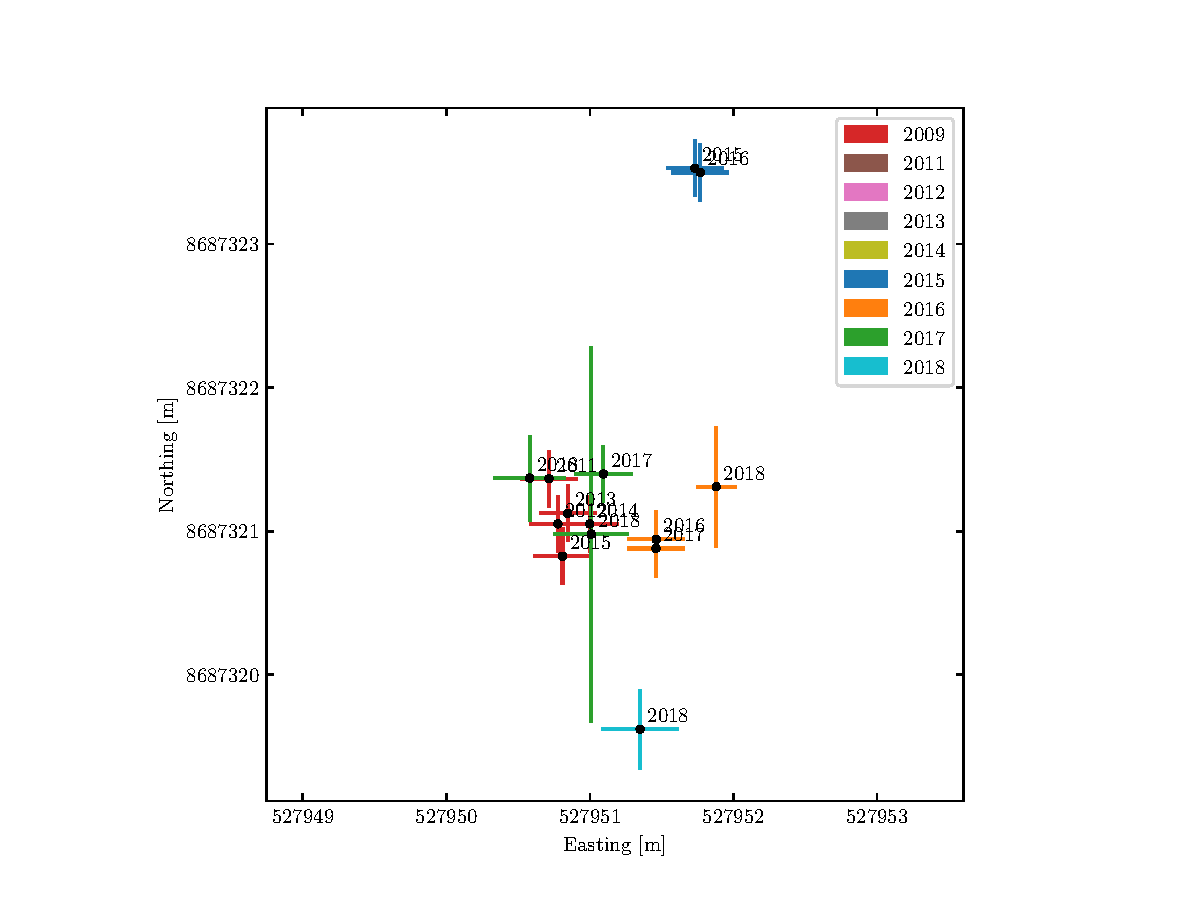
\includegraphics[width=.9\textwidth]{./figs/T2_2d.pdf}
    \caption{Present and past positions of stakes at location T2.}
    \label{GPS:fig:T2_2d}
\end{figure}

\begin{figure}[H]
    \centering
    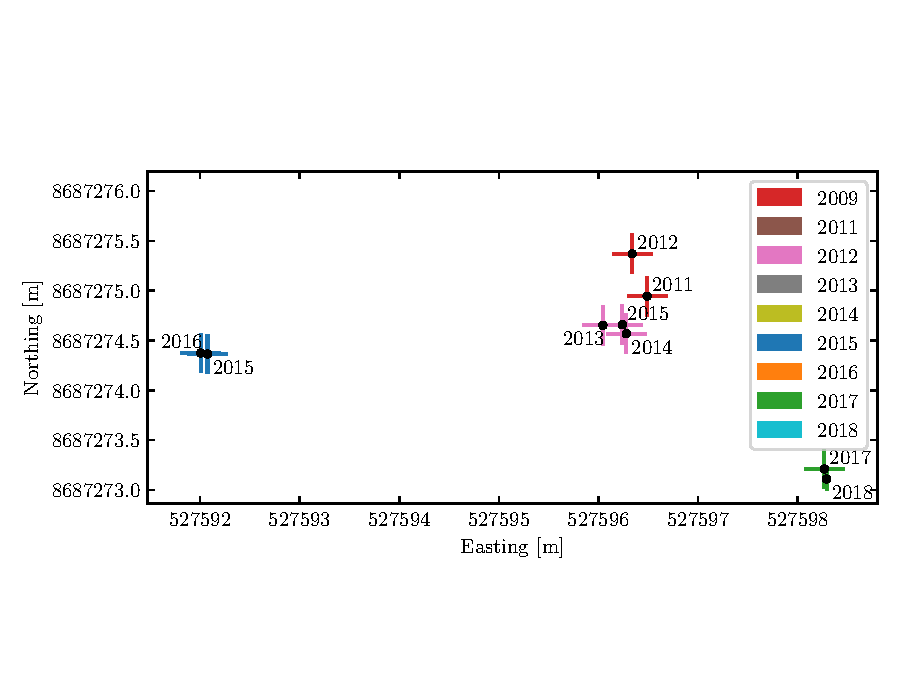
\includegraphics[width=.9\textwidth]{./figs/T3_2d.pdf}
    \caption{Present and past positions of stakes at location T3.}
    \label{GPS:fig:T3_2d}
\end{figure}

\begin{figure}[H]
    \centering
    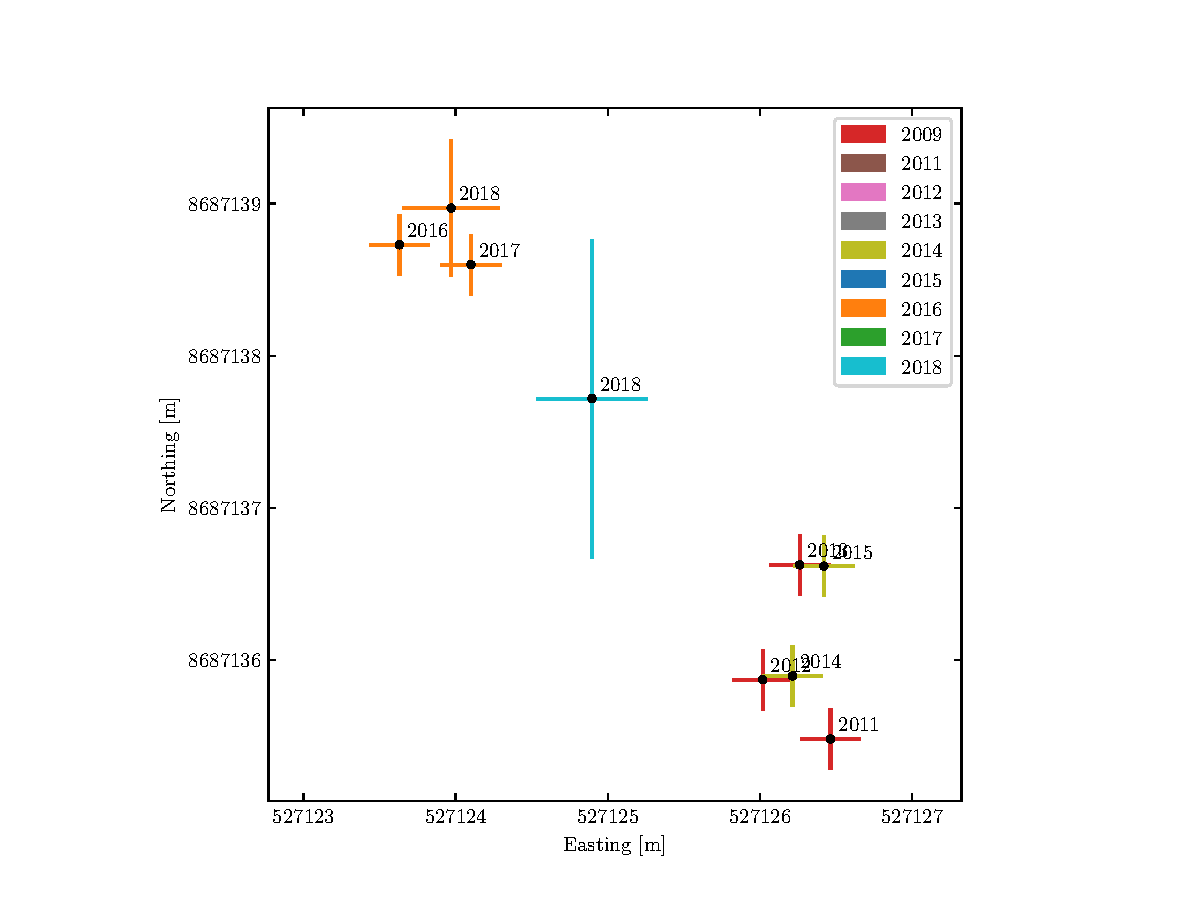
\includegraphics[width=.9\textwidth]{./figs/T4_2d.pdf}
    \caption{Present and past positions of stakes at location T4.}
    \label{GPS:fig:T4_2d}
\end{figure}

\begin{figure}[H]
    \centering
    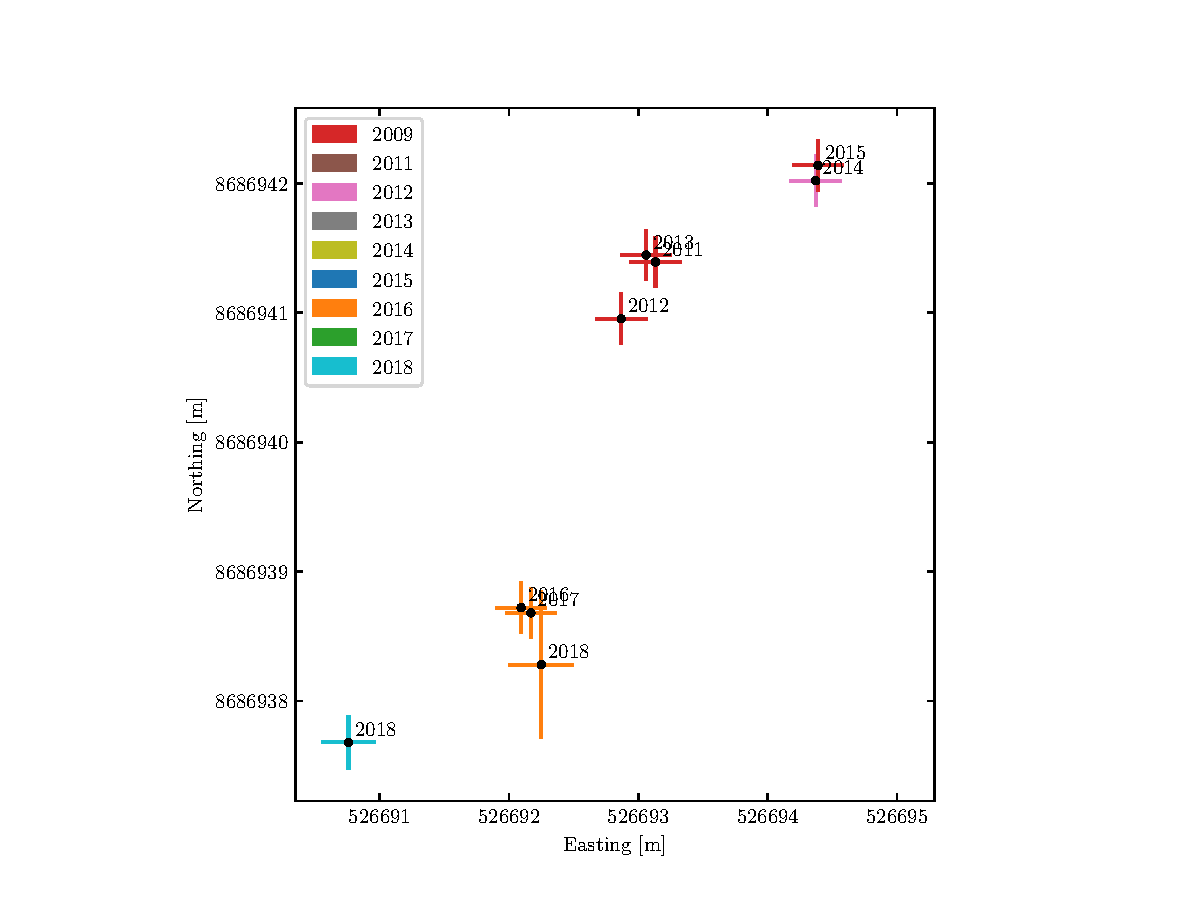
\includegraphics[width=.9\textwidth]{./figs/T5_2d.pdf}
    \caption{Present and past positions of stakes at location T5.}
    \label{GPS:fig:T5_2d}
\end{figure}

\begin{figure}[H]
    \centering
    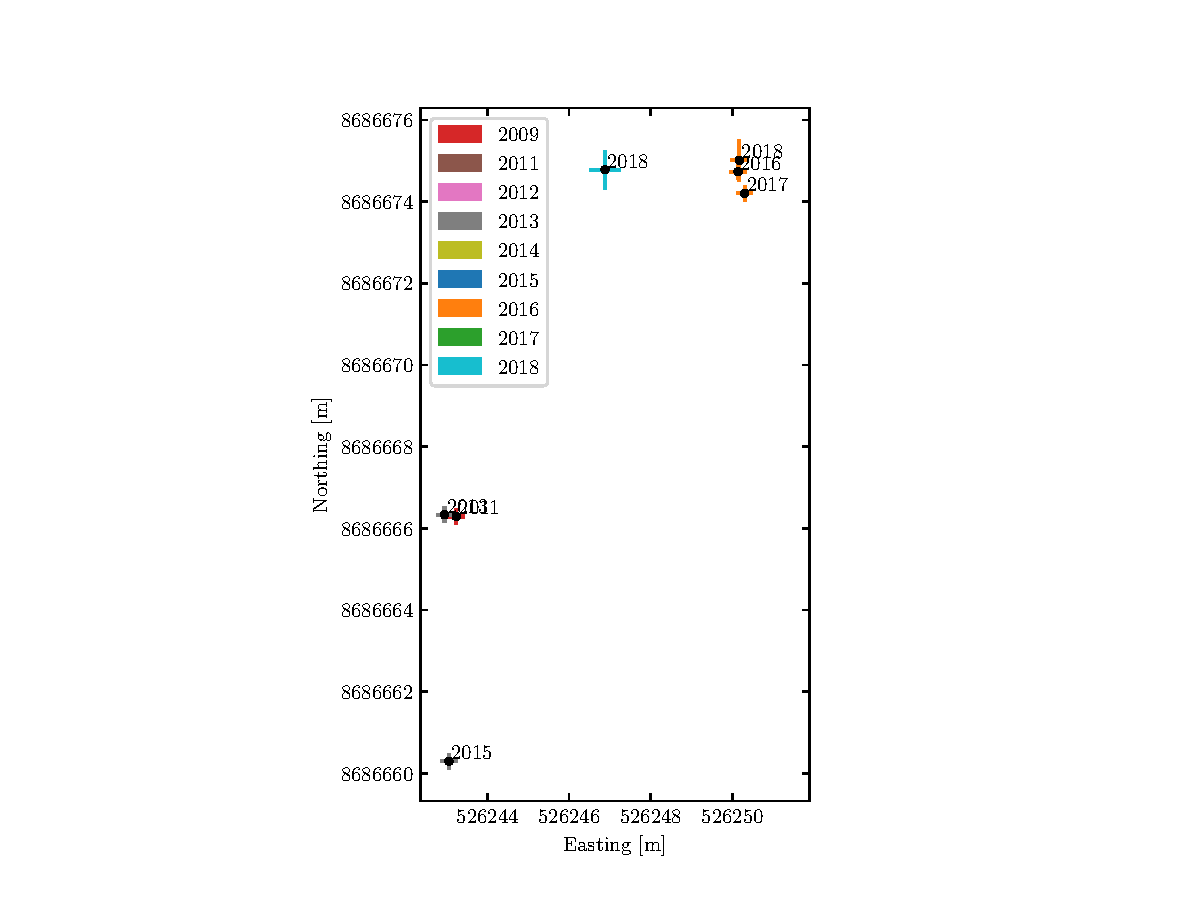
\includegraphics[width=.9\textwidth]{./figs/T6_2d.pdf}
    \caption{Present and past positions of stakes at location T6.}
    \label{GPS:fig:T6_2d}
\end{figure}

\begin{figure}[H]
    \centering
    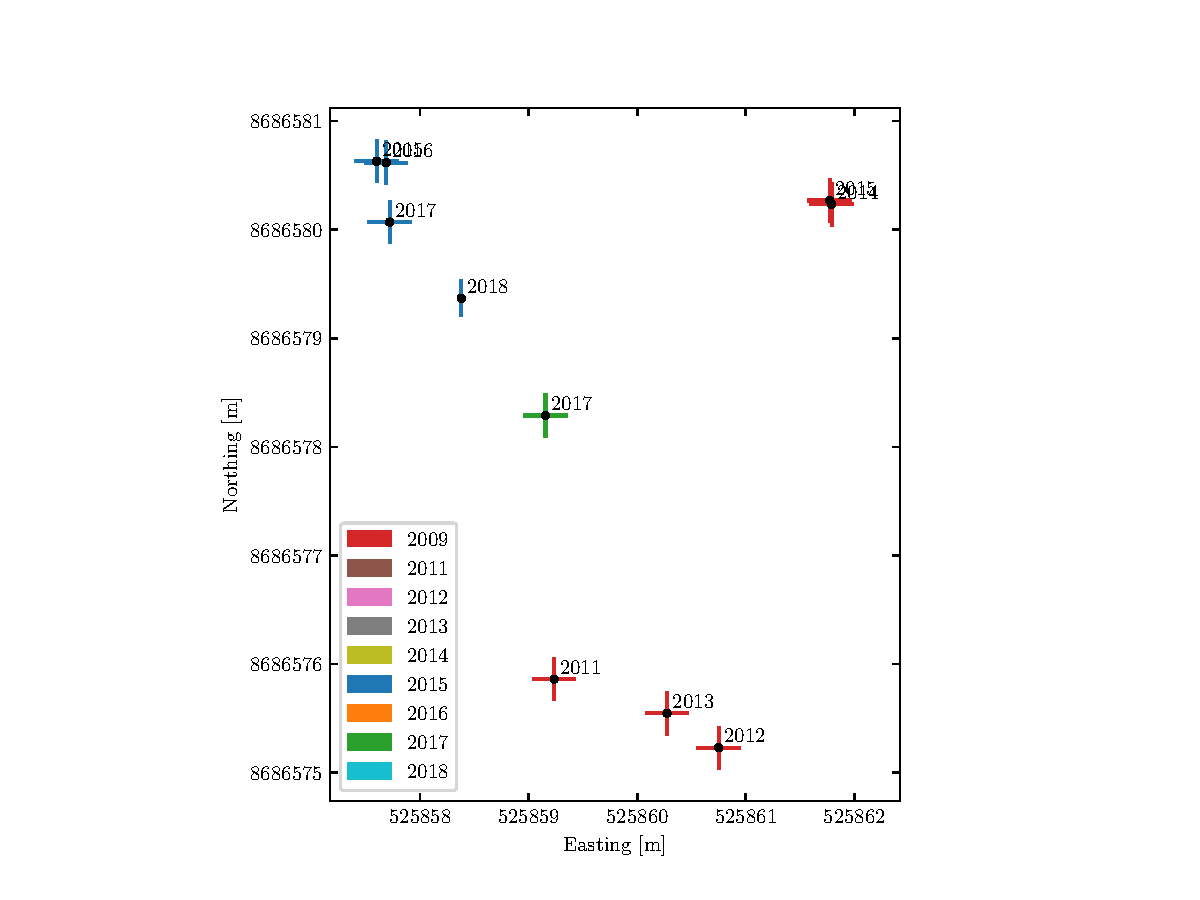
\includegraphics[width=.9\textwidth]{./figs/T7_2d.pdf}
    \caption{Present and past positions of stakes at location T7.}
    \label{GPS:fig:T7_2d}
\end{figure}

\begin{figure}[H]
    \centering
    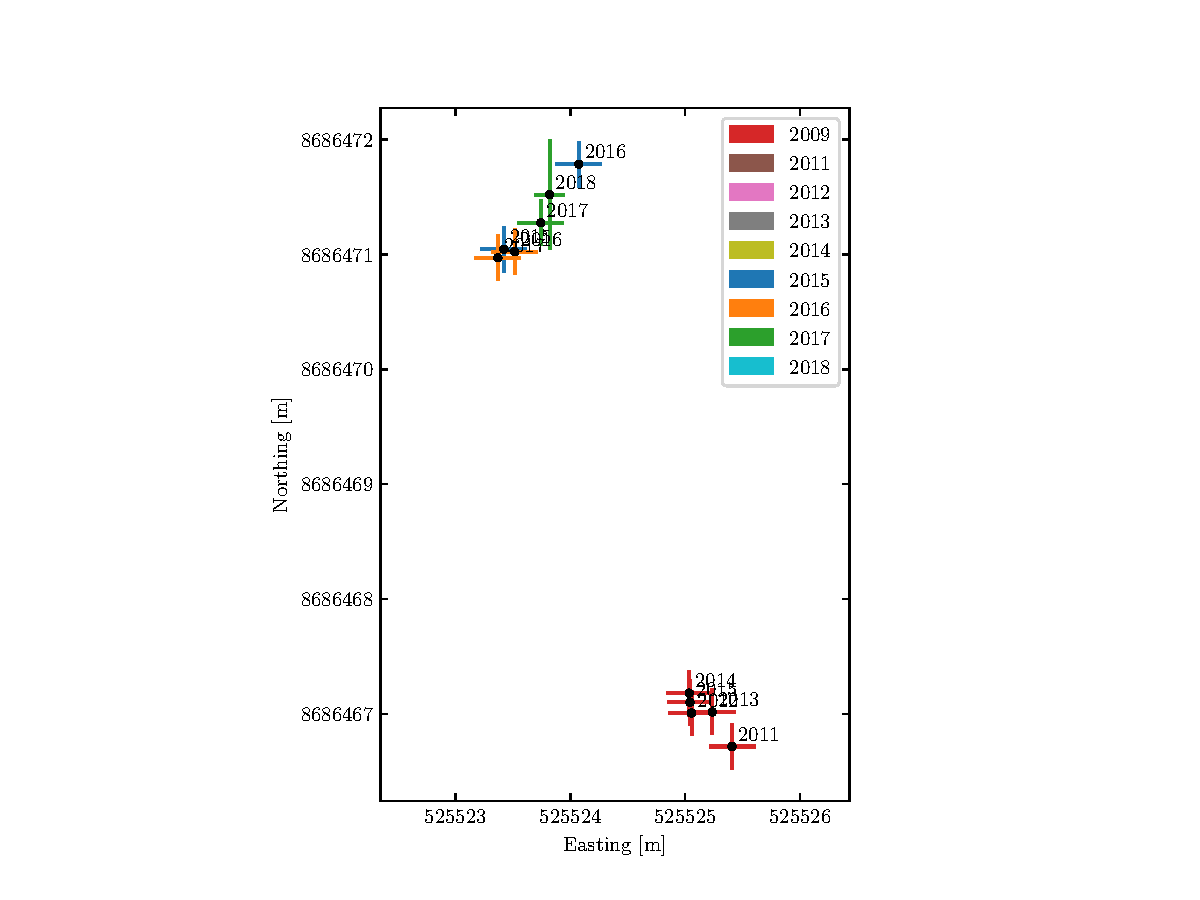
\includegraphics[width=.9\textwidth]{./figs/T8_2d.pdf}
    \caption{Present and past positions of stakes at location T8.}
    \label{GPS:fig:T8_2d}
\end{figure}

\begin{figure}[H]
    \centering
    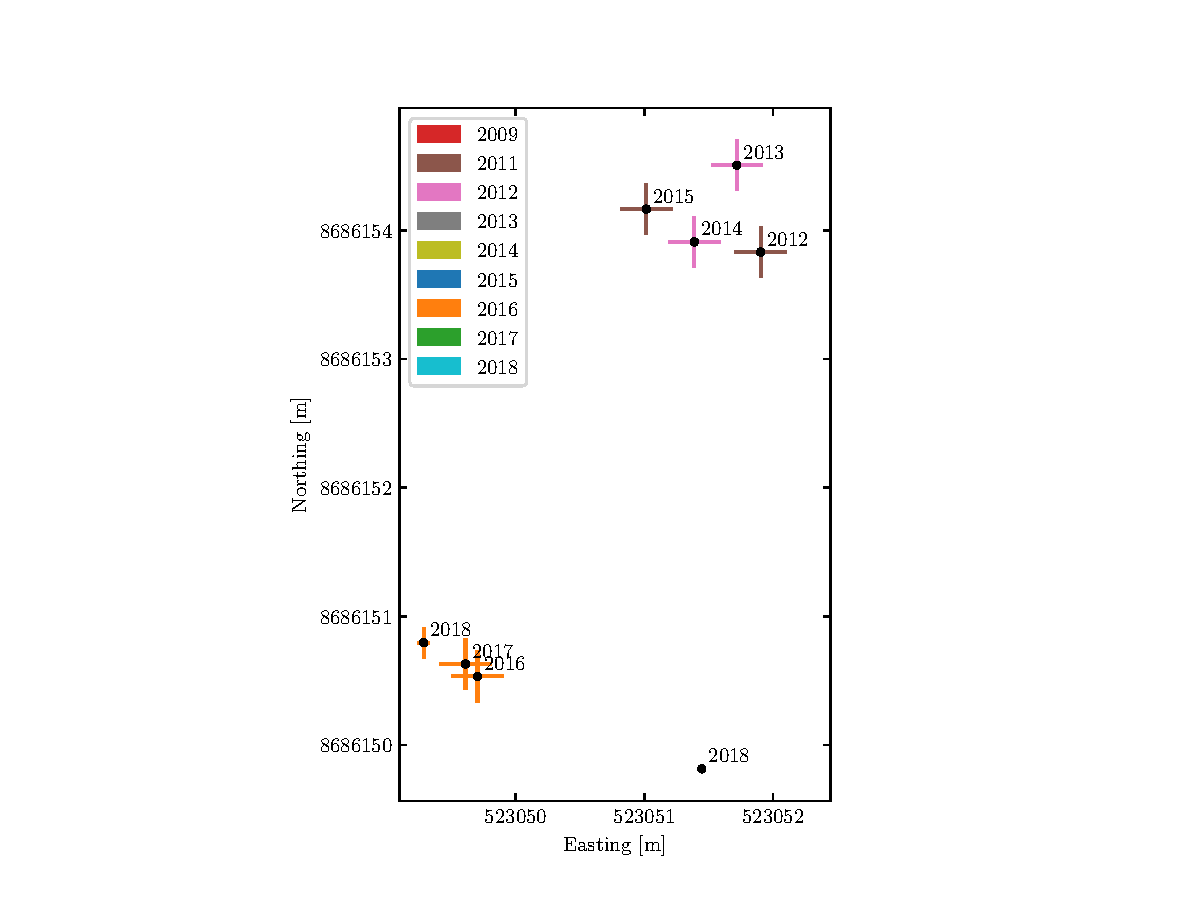
\includegraphics[width=.9\textwidth]{./figs/BL2_2d.pdf}
    \caption{Present and past positions of stakes at location BL2.}
    \label{GPS:fig:BL2_2d}
\end{figure}

\begin{figure}[H]
    \centering
    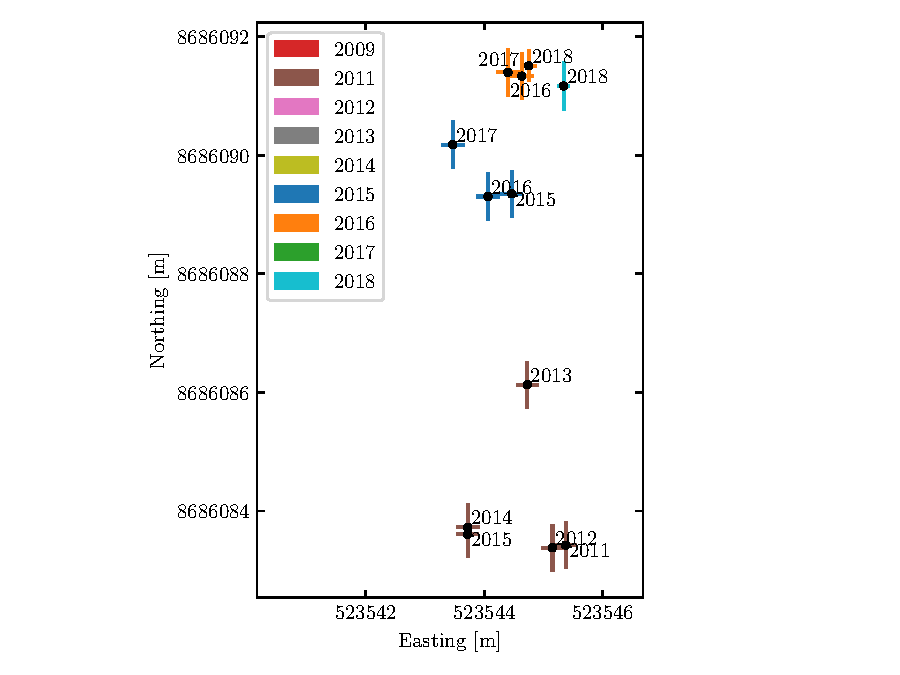
\includegraphics[width=.9\textwidth]{./figs/BL3_2d.pdf}
    \caption{Present and past positions of stakes at location BL3.}
    \label{GPS:fig:BL3_2d}
\end{figure}

\begin{figure}[H]
    \centering
    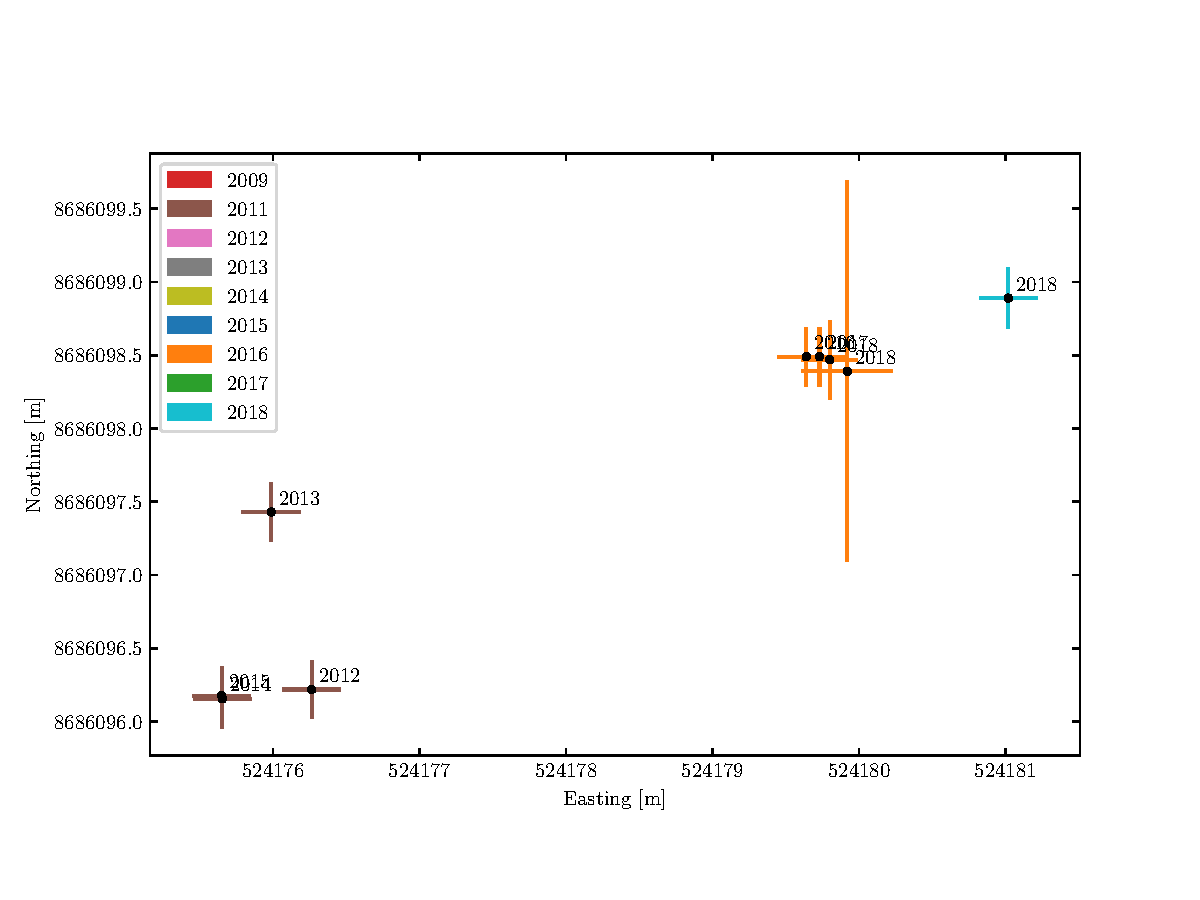
\includegraphics[width=.9\textwidth]{./figs/BL4_2d.pdf}
    \caption{Present and past positions of stakes at location BL4.}
    \label{GPS:fig:BL4_2d}
\end{figure}

\begin{figure}[H]
    \centering
    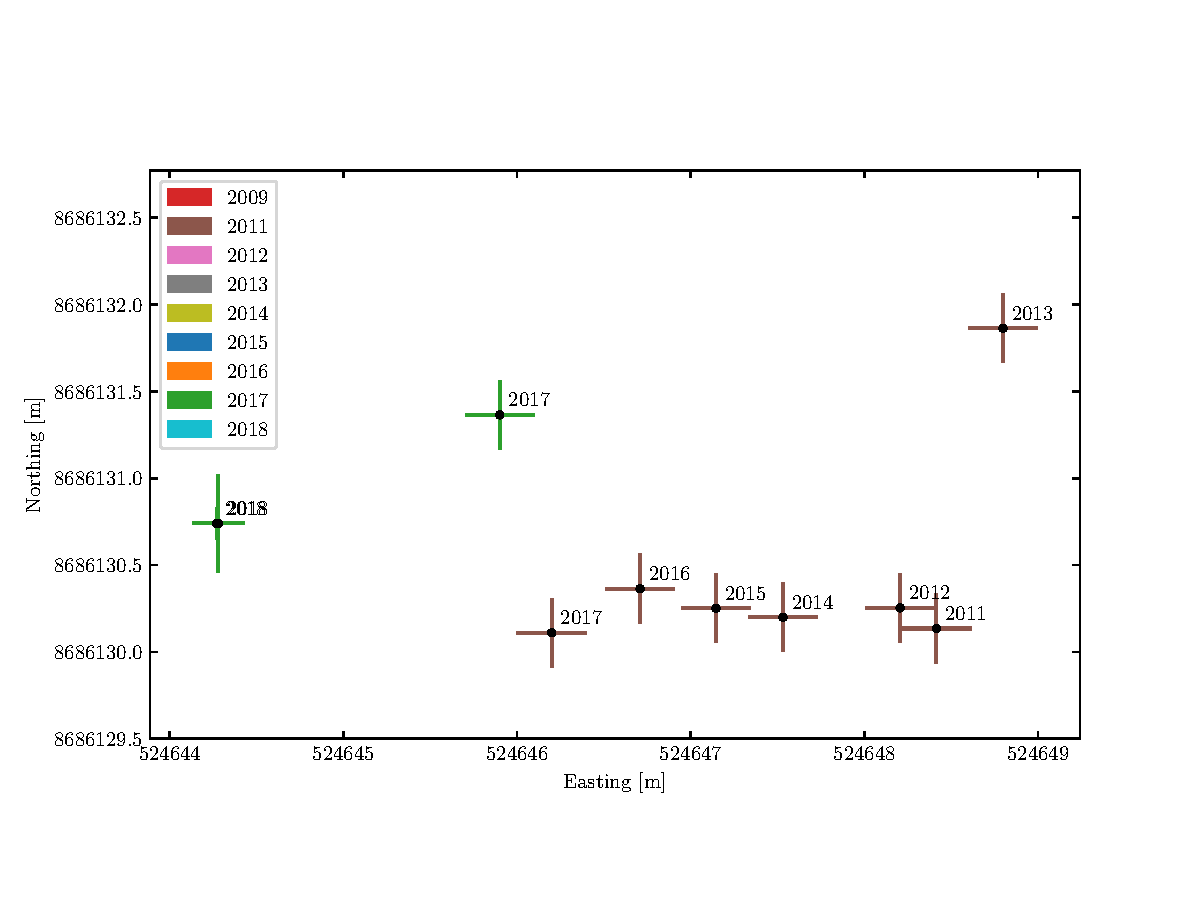
\includegraphics[width=.9\textwidth]{./figs/BL5_2d.pdf}
    \caption{Present and past positions of stakes at location BL5.}
    \label{GPS:fig:BL5_2d}
\end{figure}